% Copyright (C) 2014-2016 by Thomas Auzinger <thomas@auzinger.name>

\documentclass[draft,final]{vutinfth} % Remove option 'final' to obtain debug information.

% Load packages to allow in- and output of non-ASCII characters.
\usepackage{lmodern}        % Use an extension of the original Computer Modern font to minimize the use of bitmapped letters.
\usepackage[T1]{fontenc}    % Determines font encoding of the output. Font packages have to be included before this line.
\usepackage[utf8]{inputenc} % Determines encoding of the input. All input files have to use UTF8 encoding.

% Extended LaTeX functionality is enables by including packages with \usepackage{...}.
\usepackage{amsmath}    % Extended typesetting of mathematical expression.
\usepackage{amssymb}    % Provides a multitude of mathematical symbols.
\usepackage{mathtools}  % Further extensions of mathematical typesetting.
\usepackage{microtype}  % Small-scale typographic enhancements.
\usepackage[inline]{enumitem} % User control over the layout of lists (itemize, enumerate, description).
\usepackage{multirow}   % Allows table elements to span several rows.
\usepackage{booktabs}   % Improves the typesettings of tables.
\usepackage{subcaption} % Allows the use of subfigures and enables their referencing.
\usepackage[ruled,linesnumbered,algochapter]{algorithm2e} % Enables the writing of pseudo code.
\usepackage[usenames,dvipsnames,table]{xcolor} % Allows the definition and use of colors. This package has to be included before tikz.
\usepackage{nag}       % Issues warnings when best practices in writing LaTeX documents are violated.
\usepackage{todonotes} % Provides tooltip-like todo notes.

\usepackage{menukeys}

% fnurl adapted from http://tex.stackexchange.com/questions/115479/insert-footnotes-with-href
\usepackage{hyperref}  % Enables cross linking in the electronic document version. This package has to be included second to last.
\newcommand\fnurl[2]{%
  \href{#1}{#2}\footnote{\url{#1}}%
}

\usepackage[acronym,toc]{glossaries} % Enables the generation of glossaries and lists fo acronyms. This package has to be included last.

% Define convenience functions to use the author name and the thesis title in the PDF document properties.
\newcommand{\authorname}{Kevin Singer} % The author name without titles.
\newcommand{\thesistitle}{Title of the Thesis} % TODO The title of the thesis. The English version should be used, if it exists.
% TODO
% * a study
% * architectur
% * includes tooling
% * client side app

% Set PDF document properties
\hypersetup{
    pdfpagelayout   = TwoPageRight,           % How the document is shown in PDF viewers (optional).
    linkbordercolor = {Melon},                % The color of the borders of boxes around crosslinks (optional).
    pdfauthor       = {\authorname},          % The author's name in the document properties (optional).
    pdftitle        = {\thesistitle},         % The document's title in the document properties (optional).
    pdfsubject      = {Subject},              % The document's subject in the document properties (optional).
    pdfkeywords     = {a, list, of, keywords} % The document's keywords in the document properties (optional).
}

\setpnumwidth{2.5em}        % Avoid overfull hboxes in the table of contents (see memoir manual).
\setsecnumdepth{subsection} % Enumerate subsections.

\nonzeroparskip             % Create space between paragraphs (optional).
\setlength{\parindent}{0pt} % Remove paragraph identation (optional).

\makeindex      % Use an optional index.
\makeglossaries % Use an optional glossary.
%\glstocfalse   % Remove the glossaries from the table of contents.

% Set persons with 4 arguments:
%  {title before name}{name}{title after name}{gender}
%  where both titles are optional (i.e. can be given as empty brackets {}).
\setauthor{Pretitle}{\authorname}{Posttitle}{female}
\setadvisor{Pretitle}{Forename Surname}{Posttitle}{male}

% For bachelor and master theses:
\setfirstassistant{Pretitle}{Forename Surname}{Posttitle}{male}
\setsecondassistant{Pretitle}{Forename Surname}{Posttitle}{male}
\setthirdassistant{Pretitle}{Forename Surname}{Posttitle}{male}

% For dissertations:
\setfirstreviewer{Pretitle}{Forename Surname}{Posttitle}{male}
\setsecondreviewer{Pretitle}{Forename Surname}{Posttitle}{male}

% For dissertations at the PhD School and optionally for dissertations:
\setsecondadvisor{Pretitle}{Forename Surname}{Posttitle}{male} % Comment to remove.

% Required data.
\setaddress{Address}
\setregnumber{0123456}
\setdate{01}{01}{2001} % Set date with 3 arguments: {day}{month}{year}.
\settitle{\thesistitle}{Titel der Arbeit} % Sets English and German version of the title (both can be English or German).
\setsubtitle{Optional Subtitle of the Thesis}{Optionaler Untertitel der Arbeit} % Sets English and German version of the subtitle (both can be English or German).

% Select the thesis type: bachelor / master / doctor / phd-school.
% Bachelor:
\setthesis{bachelor}
%
% Master:
%\setthesis{master}
%\setmasterdegree{dipl.} % dipl. / rer.nat. / rer.soc.oec. / master
%
% Doctor:
%\setthesis{doctor}
%\setdoctordegree{rer.soc.oec.}% rer.nat. / techn. / rer.soc.oec.
%
% Doctor at the PhD School
%\setthesis{phd-school} % Deactivate non-English title pages (see below)

% For bachelor and master:
\setcurriculum{Media Informatics and Visual Computing}{Medieninformatik und Visual Computing} % Sets the English and German name of the curriculum.

% For dissertations at the PhD School:
\setfirstreviewerdata{Affiliation, Country}
\setsecondreviewerdata{Affiliation, Country}


\begin{document}

\frontmatter % Switches to roman numbering.
% The structure of the thesis has to conform to
%  http://www.informatik.tuwien.ac.at/dekanat

\addtitlepage{naustrian} % German title page (not for dissertations at the PhD School).
\addtitlepage{english} % English title page.
\addstatementpage

\begin{danksagung*}
\todo{Ihr Text hier.}
\end{danksagung*}

\begin{acknowledgements*}
\todo{Enter your text here.}
\end{acknowledgements*}

\begin{kurzfassung}
\todo{Ihr Text hier.}
\end{kurzfassung}

\begin{abstract}
\todo{Enter your text here.}
\end{abstract}

% Select the language of the thesis, e.g., english or naustrian.
\selectlanguage{english}

% Add a table of contents (toc).
\tableofcontents % Starred version, i.e., \tableofcontents*, removes the self-entry.

% Switch to arabic numbering and start the enumeration of chapters in the table of content.
\mainmatter

%\chapter{Introduction}
%\todo{Enter your text here.}

%\chapter{Additional Chapter}
%\todo{Enter your text here.}

% Remove following line for the final thesis.
%\input{intro.tex} % A short introduction to LaTeX.
\chapter{Introduction}

TODO -- abstract/introduction here %TODO

% use \begin{abstract}?

\chapter{Problem Description}\label{ref:probdescr}

This thesis is part of the over-arching project of crafting an
end-user-friendly
\fnurl{https://www.matchat.org/owner/}{client-application} for the
\fnurl{http://www.webofneeds.org/}{Web of Needs}
(\fnurl{http://sat.researchstudio.at/en/web-of-needs}{related
publications}), short WoN. The main focus was to research ways of
structuring the JavaScript-based client-application; thus it consisted
of researching and experimenting with state-of-the-art web-application
architectures and tooling, adapting and innovating on them for the
particular problem space, as well as identifying a migration path for
updating the existing code-base. To define the requirements, we first
need to take a high-level look over what the Web of Needs is and how
people can interact with it.

% problem-description\\
% * high-level\\
% * for people who aren't web-devs\\
% * pro problem ein satz: "prob ist im browser ld zu verwenden, dazu müssen sie geladen, geparst, gestored werden."\\

% Problemstellung (JS-Basisarchitektur für WoN-Owner App)\\
% as case study in architecture/migration\\

\todo{
define ontologies and rdf\\
\\
node = won-data/document-server\\
}


\section{Web of Needs}\label{web-of-needs}

It is a set of protocols (and reference implementations) that allow
posting documents, for instance describing supply and demand. Starkly
simplified examples would be ``I have a couch to give away'' or ``I'd
like to travel to Paris in a week and need transportation''. These
documents, called ``needs'' can be posted on arbitrary data servers
(called ``WoN-Nodes''). There they're discovered by matching-service,
that continuously crawls the nodes it finds. Additionally, to get faster
results, nodes can notify matchers of new needs. These then get compared
with the ones the matcher already knows about. If it finds a good pair
-- e.g. ``I have a couch to give away'' and ``Looking for furniture for
my living room'' -- the matcher notifies the owners of these needs. They
can then decide whether they want to contact each other. If they send
and accept each other's contact request, they can start chatting with
each other. The protocol in theory can also be used as a base-level for
other interactions, like entering into contracts or transferring money.

% PREVIOUSLY: It is a set of protocols (and reference implementations) that allow posting things like supply and demand (e.g. "I have a couch to give away") online on an arbitrary data server (called WoN-Node). These documents, called "needs", get discovered by a matching-service that notifies the owners of these needs (e.g. when the matcher finds someone that needs the couch offered). The protocols then allow for chatting (or other transactions) between the owners.

\section{Data on WoN-Nodes}\label{data-on-won-nodes}

Needs, connections between them and any events on those connections are
published on the WoN-Nodes in the form of RDF, which stands for
\fnurl{https://en.wikipedia.org/wiki/Resource_Description_Framework}{Resource
Description Framework}. In it, using a variety of different
syntax-alternatives, data is structured as a graph that can be
distributed over multiple (physical) resources. Edges in the graph in
their basic, most primitive form are described by triples of subject
(the start-node), predicates (the edge-type) and object (the
target-node). Note that subject and object need to be Unique Resource
Identifiers (URIs). Additionally, when using URIs, that also are Uniform
Resource Locators (URLs) -- together with the convention to publish data
for an RDF-node at that URL -- data-graphs on multiple servers can
easily be linked with each other, thus making them
\fnurl{https://en.wikipedia.org/wiki/Linked_data}{Linked Data}. This is a
necessary requirement for the Web of Needs, as data is naturally spread
out across several servers, i.e.~WoN-Nodes.

\begin{figure*}
\centering
\begin{verbatim}
<https://node.matchat.org/won/resource/need/7666110576054190000>
<http://purl.org/webofneeds/model#hasBasicNeedType>
<http://purl.org/webofneeds/model#Demand> .

<https://node.matchat.org/won/resource/need/7666110576054190000>
<http://purl.org/webofneeds/model#hasContent>
_:c14n0 .

<https://node.matchat.org/won/resource/need/7666110576054190000>
<http://www.w3.org/1999/02/22-rdf-syntax-ns#type>
<http://purl.org/webofneeds/model#Need> .

_:c14n0
<http://purl.org/dc/elements/1.1/title>
"Transportation Paris-Charles de Gaulle to City Center" .

_:c14n0
<http://purl.org/webofneeds/model#hasTextDescription>
"I’d like to travel to Paris in a week and need \
transportation (e.g. ride-sharing) from the airport \
to the city-center. :)" .
\end{verbatim}
\caption{Excerpt of a need description (N-Triples)}
\label{fig:needtriples}
\end{figure*}

Some example triples taken from a need description could look something
like the ones in figure \ref{fig:needtriples}.

As you can see, this way of specifying triples, called N-Triples, isn't
exactly developer-friendly; the subject is repeated and large parts of
the URIs are duplicate. The short-URIs starting with an underscore (e.g.
\texttt{\_c14n0}) are called blank-nodes and don't have a meaning
outside of a document.

There are several other mark\-up-lan\-gua\-ges res\-pec\-tively se\-ria\-li\-za\-tion-formats
for bett\-er wri\-ting and ser\-ving these tri\-ples, e.g. Tur\-tle, N3, RDF/XML and
JSON-LD. The same ex\-ample, but in Java\-Script Object No\-ta\-tion for Linked Data
(JSON-LD) would read as in figure \ref{fig:needjson}.

\todo{ TODO get syntax-highlighting to work in figures (see comment in .tex) } % \begin{lstlisting}[style=json]}
\begin{figure*}
\centering
\begin{verbatim}
{
  "@id":"need:7666110576054190000",
  "@type":"won:Need",
  "won:hasBasicNeedType":"won:Demand",
  "won:hasContent": {
    "dc:title":
      "Transportation Paris-Charles de Gaulle to City Center",
    "won:hasTextDescription":
      "I’d like to travel to Paris in a week and need transportation \
      (e.g. ride-sharing) from the airport to the city-center . :)"
  },

  "@context":{
     "need": "https://node.matchat.org/won/resource/need/",
     "rdfs":"http://www.w3.org/2000/01/rdf-schema#",
     "dc":"http://purl.org/dc/elements/1.1/",
     "won":"http://purl.org/webofneeds/model#",
     "won:hasBasicNeedType":{
        "@id":"won:hasBasicNeedType",
        "@type":"@id"
     }
  }
}
\end{verbatim}
\caption{Excerpt of a need description (JSON-LD)}
\label{fig:needjson}
\end{figure*}
% \end{lstlisting}

As you can see, JSON-LD allows to nest nodes and to define prefixes (in
the \texttt{@context}). Together this allow to avoid redundancies. The
other serialization-formats are similar in this regard (and are used
between other services in the Web of Needs); however, as JSON-LD also is
valid JSON/JS-code, it was the natural choice for using it for the
JS-based client-application.

\section{WoN-Owner-Application}\label{won-owner-application}

\subsection{Interaction Design}\label{interaction-design}

Among the three services that play roles in the web of needs --
matchers, nodes and owner-applications -- the work I did has its focus
on the latter of these. It provides people a way to interact with the
other services in a similar way that an email-client allows interacting
with email-servers. Through it, people can:

\begin{itemize}
\item
  Create and post new needs. Currently these consist of a simple
  data-structure with a subject, textual description and optional tags
  or location information.
\item
  View needs and all data in them in a human-friendly fashion
\item
  Share links to posts with other people
\item
  Immediately get notified of and see matches, incoming requests and
  chat messages
\item
  Send and accept contact/connection requests
\item
  Write and send chat messages
\end{itemize}

For exploring these interaction, several prototypes -- both paper-based
and (partly) interactive -- had already been designed, the latest of
which was a (graphical) overhaul by Ulf Harr.

\todo{ screens from last prototype }

\subsection{Technical Requirements}\label{technical-requirements}

On the development-side of things, the requirements were:

\todo{"good DX" as requirement. define it}
\begin{itemize}
\item
  Needs to be able to keep data in sync between browser-tabs running the
  JS-client and the Java-based server. This happens through a REST-API
  and websockets. Most messages arrive at the WoN-Owner-Server from the
  WoN-Node and just get forwarded to the client via the websocket. The
  only data directly stored on and fetched from the Owner-Server are the
  account details, which needs belong to an account, its key-pair and
  information on which events have been seen.
\item
  As subject of a research-project, the protocols can change at any
  time. Doing so should only cause minimal refactoring in the
  owner-application.
\item
  In the future different means of interactions between needs --
  i.e.~types need-to-need connections -- will be added. Doing so should
  only cause minimal changes in the application.
\item
  Ultimately the interface for authoring needs should support a wide
  range of ontologies respectively any ontology people might want to use
  for descriptions. Adapting the authoring guys or even just adding a
  few form input widgets should be seamless and only require a few local
  changes.
\item
  We didn't want to deal with the additional hurdles/constraints of
  designing the prototype for mobile-screens at first, but a later
  adaption/port was to be expected. Changing the client application for
  that should require minimal effort.
\end{itemize}

\todo{
TODO why we implemented it js-based:\\
* bandwith\\
* because it’s become somewhat of a wide-spread practice, i.e. “because everybody’s doing so”\\
* because there already was the angular prototype\\
* because it can run on any OS and device\\
status quo: angular app\\
}

The previous iteration of the prototype had already been implemented in
angular-js 1.X. However, the code-base was proving hard to maintain, as
we continuously had to deal with bugs that were hard to track down,
partly because JavaScript's dynamic nature obscured where they lived in
the code and mostly because causality in the angular-app became
increasingly convoluted and hard to understand. The application's
architecture needed an overhaul to deal with these issues, hence this
work you're reading. Thus, additional requirements were:

\begin{itemize}
\item
  Causality in the application is clear and concise to make
  understanding the code and tracking down bugs easier.
\item
  Local changes can't break code elsewhere, i.e.~side-effects are
  minimized.
\item
  Responsibilities of functions and classes are clear and separated, so
  that multiple developers can easily collaborate.
\item
  The current system state is transparent and easily understandable to
  make understanding causality easier.
\item
  Lessens the problems that JavaScript's weakly-typed nature causes,
  e.g.~bugs causing exceptions/errors way later in the program-flow
  instead of at the line where the problem lies.
\end{itemize}

\begin{comment}
    % TODO requirements for a full stack:
in the problem-descripion: list challenges that need to be tackled by web applications:

* seperation of concerns
  * suitability for collaboration
  * reusability of code
* move processing to client / minimal number of requests (justification for js-apps)
* networking
* optimize page load:
  * less http-requests -> bundling
  * smaller size -> minification
  * precompiling templates
* managing dependencies between scripts -> module systems
* simplicity / a low number of concepts / gentle learning curve
* predictability / maintainability


\end{comment}

\todo{
* TODO image: dependency graph in angular application\\
* slide from FB’s flux presentation?\\
* go through old application and do this empirically for a few components and bugs?\\
}





\chapter{Methods}

\begin{comment}
  <blockquote>
Methodik, die verfolgt wurde, um Lösung zu entwickeln
 -> ich glaube, den Hevner Artikel (Design Science in Inf Sys research) habe ich dir eh geschickt, eignet sich als Methode. Verbinde einfach sein abstraktes Konzept mit dem, was du tatsächliche gemacht hast (was war die Ausgangssituation (Legacy code mit Angular), wie hat dein Suchprozess ausgesehen (wie bist du auf react gekommen, was waren die Alternativen,...), Was kam aus der globalen Knowledge Base (react), wie kamst du zu deiner Synthese aus react+rdfstore-js+angular)
 </blockquote>

 <blockquote>
 in the method chapter you should explain:
* hevner
* RDF, linked data, JSON-LD
* angular
* flux/redux
 </blockquote>

 % Flo @ hevner-summary: good first note sheet. You can convert that into a 1-2 page intro of the methods section. Then you go on to show how you applied this framework, effectively proving that what you did is research, and not engineering.

 % TODO better describe/address the figure

% 2: @hevner-länge: macht nichts, aber man darf sich beim lesen nicht fragen, warum du einem das erzählstFrom:phlow_06 (Flo SAT)wenn du keinen grund dafür findest: weglassen. sonst: sagen. -- dh ich sollte e.g. auch nur die artefakt-kategorie beschreiben, unter die der prototyp / die architektur fällt, bzw die methoden, die tatsächlich verwendet wurden?(die guidelines werde ich alle brauchen, da die dann hinterher ja die struktur für den kern-teil darstellen sollen). wobei die anderen artefakt-kategorien/-abgrenzung ermöglichen --> liste an methoden kürzen

% dann bleibt das eigentlich eh bei den 3-4 seiten (atm ist es eh fast nur aufzählung + kurze definition für alles)
% From:phlow_06 (Flo SAT) genau, es fehlt glaub ich noch die erklärung, warum das jetzt aufgezählt wird - also wie du das für dich umsetzt

% TODO answer the two fundamental questions explicitly

<!--

Vorlage: Arbeit vom Roman?

## Ressources

### Redux

<https://medium.com/javascript-scene/10-tips-for-better-redux-architecture-69250425af44#.auuzhdjz3>
[You Might Not Need Redux](https://medium.com/@dan_abramov/you-might-not-need-redux-be46360cf367#.2xg3p7aef)


<!-- TODO see hevner_summary + notes !!!! -->
<!--
TODO
Technische Realisierung / solutions
  * follow hevner's structure(?)
-->
<!--
describe architecture / redux cycle here
describe entire tool-chain?
-->


From TU-outline:
* used concepts
  * redux
  * side-effects / immutable data
  * bi-directional binding
* methods and/or models
* languages
  * javascript
  * sparql?
  * json-ld
* design methods
  * hevner
  * iterations / design-cycle
* data models
* analysis methods
  * ???
  * personal experience / experience of colleagues?
* formalisms

\end{comment}

\section{Design Science in Information Systems Research}

For the work preceding this thesis the methodological
framework presented in ``Design Science in Information
Systems Research'' by Hevner et al (2004) was used.
I'll try to give a short overview over it in this section.

\subsection{Design Science}

The paper states that a lot of the research surrounding information systems can be described as design- and/or behavioral science.

It roughly defines \textbf{behavioral science} with regard to IS-research as concerned with the analysis of the interactions of people and technology, with the goal of uncovering ``truths'' and predicting or explaining phenomena surrounding these interactions.

In comparison, Hevner et al describe \textbf{design science} as concerned with problem solving and construction with the background that doing so leads to understanding the addressed ``wicked'' problem \footnote{\label{ref:wicked}Here, ``wicked'' problems (Brooks 1987, 1996; Rittel, Webber 1984) are defined as those with unstable requirements, ill-defined environmental contexts, complex interactions among subcomponents of problem and solution, an inherent flexibility to change design processes and artifacts and a critical dependence on human cognitive abilities (e.g. creativity) and social abilities (e.g. teamwork) for effective solutions}. It diffentiates itself from \textbf{routine design} by addressing problems without existing best-practices/requisite knowledge and solves them unique/innovative ways, or improves efficiency. By doing so, new knowledge is contributed to the foundations and methodolgies. Design-science usually also produces prototypes instead of full-grown systems.



% TODO replace references to wicked problems with glossary entry
% foobar \glspl{wicked}
% \newglossaryentry{wicked}
% {
  % name={wicked problem},
  % description={These are defined in  Brooks 1987, 1996 and Rittel, Webber 1984 as problems with unstable requirements, ill-defined environmental contexts, complex interactions among subcomponents of problem and solution, an inherent flexibility to change design processes and artifacts and a critical dependence on human cognitive abilities (e.g. creativity) and social abilities (e.g. teamwork) for effective solutions}
% }

The paper also presents two \textbf{fundamental questions} of design research as ``What utility does the new artifact provide?'' and ``What demonstrates that utility?''. As all other's from Hevner et al (2004) that are referenced or quoted here, they'll be addressed in the next chapter. %TODO more concrete/pinpointed reference

\subsection{Design Processes and Artifacts}


March and Smith (1995)\footnote{TODO} list two processes involved in design, \textbf{build/generate} and \textbf{evaluate}, that form a cycle (see figure \ref{fig:hevner}). They differentiate the artifacts produced as:

\begin{description}
 \item[constructs] that provide the language to define problems and solutions (e.g. programming languages)
 \item[models] that abstract and represent these and allow exploring the effects of design decisions
 \item[methods] that define how to solve problems or aid with searching the problem-space (e.g. algorithms, best practices)
 \item[instantiations] that demonstrate feasibility and enable assessing suitability for the intended purpose
\end{description}

\subsection{Design-Science Research Guidelines}

\begin{figure*}
\centering
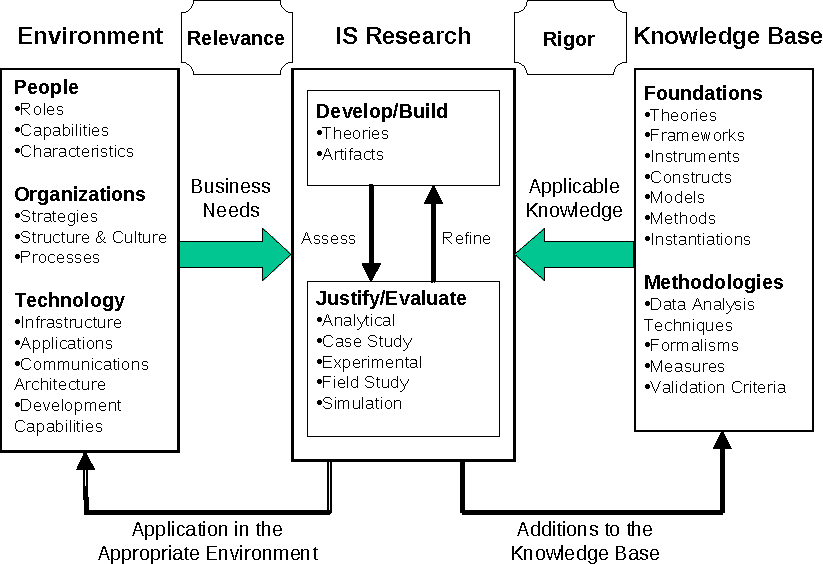
\includegraphics[width=1.0\textwidth]{figures/Hevner-et-al-2004-figure-2.pdf}
\caption{\label{fig:hevner}Information Systems Research Framework (Hevner et al 2004)}
\end{figure*}

Hevner et al (2004) defines seven guidelines that design-science in information systems should address (but not necessarily come-what-may adhere to), which will be done in the next chapter. % TODO more conrete/clickable reference
They are as follows:

% TODO
% \begin{leftbar}
%  asdf
%  asdf
%\begin{leftbar}

%\begin{siderules}
%\begin{quotation}
\begin{description}

\item[Design as an Artifact]
``Design-science research must produce a viable artifact in the form of a construct, a model, a method, or an instantiation.'' This allows to demonstrate feasibility -- for cases where that wasn't a given yet -- thus making it research (as opposed to routine design).

% This

\item[Problem Relevance]
``The objective of design-science research is to develop technology-based solutions to important and relevant business problems.'' Relevancy here is with respect to a  ``constituent community'' (e.g. IS practitioners)
% TODO mention Technology Acceptance Model here (and need to define it)? i haven't really done anything based on it, so whatever

\item[Design Evaluation]
``The utility, quality, and efficacy of a design artifact must be rigorously demonstrated via well-executed evaluation methods.'' This usually requires integration into the usage context (to see if it ``works'' there or is ``good'' in it), the definition of appropriate metrics and gathering of appropriate data. Evaluation provides valueable and necessary feedback for the design iterations (see figure \ref{fig:hevner})

\item[Research Contributions]
``Effective design-science research must provide clear and verifiable contributions in the areas of the design artifact, design foundations, and/or design methodologies.'' Important here is the novelty of the artifact -- by extending or innovatively (re-)applying previous knowledge -- as well as its generality and significance.

\item[Research Rigor]
``Design-science research relies upon the application of rigorous methods in both the construction and evaluation of the design artifact.'' This means applying existing foundations and methodologies, using effective metrics and formalising. Note, however, that an overemphasis on rigor can often lead to lower relevance (Lee 1999), as many environments and artifacts defy an excessive formalism (see ``wicked problems'' at footnote \ref{ref:wicked}). %TODO better reference / use glossary entry

\item[Design as a Search Process]
``The search for an effective artifact requires utilizing available means to reach desired ends while satisfying laws in the problem environment.'' This entails using heuristic search stragegies (e.g. best-practices as starting point) in ght generate/test-cycle (see figure \ref{fig:hevner}) However, again, it might not be possible to formalize or even determine any of these, due to the ``wicked'' (see footnote \ref{ref:wicked}) nature of tackled problems. As a result it might often be necessary to only work on simpler sub-problems, giving up relevancy in turn.

\item[Communication of Research]
``Design-science research must be presented effectively both to technology-oriented as well as management-oriented audiences.'' For the former the construction and evaluation process are important (e.g. to allow reproduction). For the latter the question boils down to ``Is it worth the effort to use the artifact for my business?''. This can be broken down as ``What knowledge is required?'' respectively ``Who can use it?'', ``How imporant is the problem?'', ``How effective is the solution?'' as well as some details in appendicesto appreciating the work.

\end{description}
%\end{quotation}
%\end{siderules}



\subsection{Design Evaluation Methods}

\begin{comment}
% TODO drop methods that weren't used

% TODO metrics from "Design Evaluation:"
  * evaluate in terms of:
    * functionality
    * completeness
    * consistency
    * accuracy
    * performance
    * reliability
    * usability
    * fit with the organization
    * other relevant quality attributes
* establish if it does work and in which environments
  * what constitutes “working” and “good”? which metrics?
  * compare with other solutions for the same problem by human experts
\end{comment}

Observational methods:

\begin{description}
  \item[Case Study] ``Study artifact in depth in business environment''
    % * **{** ^ that **}**
    % * **{** anecdotal evidence by fsu/fk/sbyim/yp how they feel about it? (super-biased due to interaction with me) **}**
  \item[Field Study] ``Monitor use of artifact in multiple projects''
    % * **{** the meinkauf app! what did we use there? ionic and vanilla angular or ng-redux too? <!-- TODO get copy of mk repo --> **}**
\end{description}

Analytical methods:

\begin{description}
  \item[Static Analysis] ``Examine structure of artifact for static qualities (e.g., complexity)''
    % * **{** graph out dependencies in both apps, if necessary in one vertical slice of one process <!-- TODO make graph of dependencies -->  **}**
    % * **{** code-examples of very simple apps with both architectures to demonstrate boiler-plate / overhead? Todo-MVC? <!-- TODO write examples -->  **}**
  \item[Architecture Analysis] ``Study fit of artifact into technical IS architecture''
    % * **{** analyze how well it interacts with the rest of the WoN-ecosystem. what defines “interacts well”? <!-- TODO ponder --> **}**
  \item[Optimization] ``Demonstrate inherent optimal properties of artifact or provide optimality bounds on artifact behavior''
  \item[Dynamic Analysis] ``Study artifact in use for dynamic qualities (e.g., performance)''
\end{description}

Experimental Methods:

\begin{description}
  \item[Controlled Experiment] ``Study artifact in controlled environment for qualities (e.g., usability)''
  \item[Simulation] ``Execute artifact with artificial data''
\end{description}

Testing:

\begin{description}
  \item[Functional (Black Box) Testing] ``Execute artifact interfaces to discover failures and identify defects''
  \item[Structural (White Box) Testing] ``Perform coverage testing of some metric (e.g., execution paths) in the artifact implementation''
\end{description}

Descriptive Methods:

\begin{description}
  \item[Informed Argument] ``Use information from the knowledge base (e.g., relevant research) to build a convincing argument for the artifact’s utility''
    % * **{** ^ this **}**
    % TODO: ^ (only) usable for more innovative artifacts for which other methods aren’t feasible
  \item[Scenarios] ``Construct detailed scenarios around the artifact to demonstrate its utility''
\end{description}

% \input{03_02.tex}


\backmatter

% Use an optional list of figures.
\listoffigures % Starred version, i.e., \listoffigures*, removes the toc entry.

% Use an optional list of tables.
\cleardoublepage % Start list of tables on the next empty right hand page.
\listoftables % Starred version, i.e., \listoftables*, removes the toc entry.

% Use an optional list of alogrithms.
\listofalgorithms
\addcontentsline{toc}{chapter}{List of Algorithms}

% Add an index.
\printindex

% Add a glossary.
\printglossaries

% Add a bibliography.
\bibliographystyle{alpha}
\bibliography{intro}

\end{document}
